\documentclass[../main.tex]{subfiles}
\begin{document}
\lstset{language=Matlab}
\section*{Introduction}
In this assignment, our goals are to
\begin{itemize}
\item implement 3-node and 6-node triangular membrane elements
\item implement assembly of force and stiffness matrices for a mesh of
  these elements
\item implement finite element analysis of some example problems using
  the membrane elements
\end{itemize}
\section{Finite Element Formulation of a Membrane}
Membrane theory can be derived from shell theory with the assumption
that the shell is very thin and does not offer resistance to bending
or transverse shear. We also assume that behaviour of the membrane
through its thickness is same as that for the mid-surface and hence it
is sufficient to calculate the behaviour of just the mid-surface. The
change in the thickness direction can be represented by a single
parameter, the thickness stretch, $\lambda$.

Let $\mathbf{a}$ and $\mathbf{A}$ denote the curvilinear basis vectors
in the current and reference configurations of the mid-surface
respectively. If $x_{ia}$ and $X_{ia}$ denote the co-ordinates of the
nodes of the triangular membrane element in current and reference
configuration respectively then tangent basis vectors in curvilinear
frame are given as
\begin{align*}
  a_\alpha &= \mathbf{x}_{,\alpha}=x_{ia}N_{a,\alpha} \\
  A_\alpha &= \mathbf{X}_{,\alpha}=X_{ia}N_{a,\alpha}
\end{align*}
where $N_{a}$ are the shape functions for triangular elements derived
in HW 2 and $\alpha = 1,2$. The third curvilinear tangent basis vector
is assumed to always be normal to the other two. This means,
\begin{align*}
  \mathbf{a}_3 &= \frac{\mathbf{a}_1\times \mathbf{a}_2}{\lvert \mathbf{a}_1\times \mathbf{a}_2\rvert}\\
  \mathbf{A}_3 &= \frac{\mathbf{A}_1\times \mathbf{A}_2}{\lvert \mathbf{A}_1\times \mathbf{A}_2\rvert}
\end{align*}
For further calculations, we require the dual basis vectors in the
refernce configuration of mid-surface, $\mathbf{A}^i$. These can be
derived as follows
\begin{align*}
  A_{ij} &= \mathbf{A}_i\cdot \mathbf{A}_j \\
  A^{ij} &= A_{ij}^{-1}\\
  \mathbf{A}^i &= A^{ij}\mathbf{A}_j
\end{align*}
where $A_{ij}$ is the metric tensor and $A^{ij}$ is the inverse metric
tensor. It should be pointed out that as a consequence of our
assumptions in membrane theory we have $\mathbf{A}_3 = \mathbf{A}^3$.
\subsection{Deformation Gradient}
Using the curvilinear basis vectors derived in the previous section we
can write the deformation gradient of the element as
\begin{align*}
  \mathbf{F} = \mathbf{a}_\alpha\otimes \mathbf{A}^{\alpha} + \lambda \mathbf{a}_3\otimes \mathbf{A}^3
\end{align*}
where $\lambda$ is the thickness stretch ratio. We need to provide an
initial guess for $\lambda$ to start with. Then, using the deformation
gradient and the Lam\'{e} coefficients, we can calculate strain energy
density, $w$, the first Piola-Kirchhoff stress tensor $\mathbf{P}$ and
the stiffness modulus $C_{iJkL}$ based on the compressible neo-Hookean
constitutive model developed in HW 1. Now, we are in position to
implement plane stress condition for the triangular element.
\subsection{Plane-stress condition}
The component of traction vector in the direction of surface normal in
the current configuration can be written as
\begin{align*}
  T(\lambda) = \mathbf{a}_3\cdot\left(\mathbf{P}(\lambda)\mathbf{A}_3\right)
\end{align*}
To enforce planes stress we need to solve for $\lambda$ such that
$T(\lambda) = 0$. We will use Newton-Raphson method to solve for
$\lambda$. We need Taylor series expansion of $\mathbf{P}(\lambda)$
and $T(\lambda)$.
\begin{align*}
  \mathbf{P}(\lambda+d\lambda) &\approx \mathbf{P}(\lambda) + \frac{\partial \mathbf{P}}{\partial \lambda}\mathrm{d}\lambda\\
                               &= \mathbf{P}(\lambda) + \frac{\partial\mathbf{P}}{\partial\mathbf{F}}:\frac{\partial\mathbf{F}}{\partial\lambda}\mathrm{d}\lambda\\
                               & = \mathbf{P}(\lambda) + \mathbb{C}:\frac{\partial\mathbf{F}}{\partial\lambda}\mathrm{d}\lambda\\
                               &=\mathbf{P}(\lambda) + \mathbb{C}:(\mathbf{a}_3\otimes\mathbf{A}^3)\mathrm{d}\lambda
\end{align*}
Therefore,
\begin{align*}
  T(\lambda+\mathrm{d}\lambda) &\approx \mathbf{a}_3\cdot\left(\mathbf{P}(\lambda+\mathrm{d}\lambda)\mathbf{A}_3\right)\\
                               &= T(\lambda) + \mathbf{a}_3\cdot\left(\mathbb{C}:(\mathbf{a}_3\otimes\mathbf{A}^3)\mathbf{A}^3\right)\mathrm{d}\lambda\\
                               & = T(\lambda) + (\mathbf{a}_3\otimes\mathbf{A}^3):\mathbb{C}:(\mathbf{a}_3\otimes\mathbf{A}^3)\mathrm{d}\lambda
\end{align*}
If $T(\lambda+\mathrm{d}\lambda) = 0$ then
\begin{align*}
  \mathrm{d}\lambda = - T(\lambda)\left[(\mathbf{a}_3\otimes\mathbf{A}^3):\mathbb{C}:(\mathbf{a}_3\otimes\mathbf{A}^3)\right]^{-1}
\end{align*}
This gives the update to $\lambda$ for the Newton-Raphson
interations. The term in the bracket is $C_{3333}$, component of
stiffness modulus in the curvilinear frame. It can be computed in
terms of $C_{iJkL}$ which is in the lab-frame as
\begin{align*}
  C_{3333} = (\mathbf{a}_3)_i(\mathbf{A}_3)_JC_{iJkL}(\mathbf{a}_3)_k(\mathbf{A}_3)_L
\end{align*}
\subsection{Strain Energy }
After solving for $\lambda$ using Newton-Raphson method for plane
stress, we can re-calculate $\mathbf{F}$. Thus, we can calculate
strain energy density, $w$, as per the compressible neo Hookean
constitutive model of HW 2. The strain energy of the element, $W$, can
be written as
\begin{align*}
  W &= \int_{V^e}\!w\, \mathrm{d}V^e\\
    &=\int_{\Omega^e}\!w\,\mathrm{d}\Omega^eH\\
\end{align*}
where $H$ is membrane thickness and $\Omega$ is the mid-surface. We
need to evaluate the integral using Gauss quadrature for triangular
region developed in HW 2. Let $n_G$ be the number of Gauss quadrature
points, $\hat{\Omega}$ be the area of standard parametric triangle and
$\hat{w}$ be the weight for the Gauss quadrature point. Then we can
write
\begin{align*}
  W &=\int_{\Omega^e}\! w \, \mathrm{d}\Omega^eH\\
    &=\int_{\hat{\Omega}}\! wH\sqrt{A} \, \mathrm{d}\hat{\Omega}\\
    &=\sum_{q=1}^{n_G}w\hat{w}_qH\sqrt{A}\hat{\Omega}
\end{align*}
where $A = \lvert A_{ij}\lvert$ is determinant of the metric tensor.
\subsection{Internal and External Forces}
The internal nodal forces can be written in terms of stress-resultant
$\mathbf{n}^{\alpha}$.
\begin{align*}
  \mathbf{n}^{\alpha} &= \mathbf{P}\cdot\mathbf{A}^{\alpha} H \\
\end{align*}
The internal forces are
\begin{align*}
  f_{ia}^{\text{int}} &= \int_{\hat{\Omega}}\! n_i^{\alpha}N_{a,\alpha}\sqrt{A} \, \mathrm{d}\hat{\Omega}\\
                      &=\sum_{q=1}^{n_G}n_i^{\alpha}N_{a,\alpha}\bigg\lvert_{\theta_q}\hat{w}_q\sqrt{A}\hat{\Omega}
\end{align*}
The external forces are obtained from the distributed transverse load
on the element, $\mathbf{f}$,
\begin{align*}
  f_{ia}^{\text{ext}} &= \int_{\hat{\Omega}}\! f_iN_a\sqrt{A}\, \mathrm{d}\hat{\Omega}\\
                      &=\sum_{q=1}^{n_G}f_iN_a\bigg\lvert_{\theta_q}\hat{w}_q\sqrt{A}\hat{\Omega}
\end{align*}
\subsection{Stiffness Modulus}
To calculate the element stiffness modulus, $K_{iakb}$, we need to
calculate the curvilinear components of Kirchhoff stress tensor,
$\bm{\tau}$,
\begin{align*}
  \bm{\tau} &= \mathbf{P}\mathbf{F}^T\\
            &= \mathbf{F}(\mathbf{F}^{-1}\mathbf{P})\mathbf{F}^{T}\\
            &= \mathbf{F}\mathbf{S}\mathbf{F}^{T}
\end{align*}
where $\mathbf{S}=\mathbf{F}^{-1}\mathbf{P}$ is the second
Piola-Kirchhoff stress tensor. $\mathbf{S}$ and $\bm{\tau}$ have the
same components but different basis vectors. The relationship can be
written as
\begin{align*}
  \mathbf{S} = \tau^{\alpha\beta}\mathbf{A}_{\alpha}\otimes\mathbf{A}_{\beta}
\end{align*}
where $\tau^{\alpha\beta}$ are the components of $\bm{\tau}$ in the
curvilinear frame which can be obtained as
\begin{align*}
  \tau^{\alpha\beta} &= \mathbf{A}^\alpha\cdot\left(\mathbf{S}\mathbf{A}^{\beta}\right)
\end{align*}
We also need the components of stiffness modulus in terms of
$\bm{\tau}$
\begin{align*}
  C^{ijkl} = \frac{\partial\tau^{ij}}{\partial a_{kl}}
\end{align*}
where $a_{kl}$ are components of metric tensor in current
configuration. We can obtain this using the stiffness modulus in terms
of the second Piola-Kirchoff stress tensor
\begin{align*}
  C_{IJKL} = \frac{\partial S_{IJ}}{\partial C_{KL}}
\end{align*}
where $C_{KL}$ are components of the left Cauchy Green strain
tensor. We can calculate $C_{IJKL}$ from $C_{iJkL}$ which is the
stiffness modulus in terms of the first Piola-Kirchoff stress tensor.
\begin{align*}
  C_{IJKL} = \frac{1}{2}F^{-1}_{Ii}F^{-1}_{Kk}\left(C_{iJkL}-\delta_{ik}S_{JL}\right)
\end{align*}
Now,
\begin{align*}
  C^{ijkl} = C_{IJKL}(\mathbf{A}^i)_I(\mathbf{A}^j)_J(\mathbf{A}^k)_K(\mathbf{A}^l)_L
\end{align*}
where $\left(\cdot\right)_I$ represents the $I^{th}$ component in
lab-frame of the vector in the brackets. When we impose the
plane-stress condition, we force $\tau^{33} = 0$. This requires
modifying $C^{\alpha\beta\gamma\delta}$ such that it is consistent,
that is, it can be obtained by differentiating $\tau^{\alpha\beta}$
with respect to $a^{\gamma\delta}$. The modified form is given as
\begin{align*}
  \tilde{C}^{\alpha\beta\gamma\delta} = C^{\alpha\beta\gamma\delta} - \frac{C^{\alpha\beta33}}{C^{3333}}C^{33\gamma\delta}
\end{align*}
Now we have all components we need to write the element stiffness
modulus.
\begin{align*}
  K_{iakb} &= \underbrace{\int_{\hat{\Omega}}\! \left(\tilde{C}^{\alpha\beta\mu\nu}(\mathbf{a}_\beta\otimes\mathbf{a}_\nu)_{ik}N_{a,\alpha}N_{b,\mu}\right)\sqrt{A} \,\mathrm{d}\hat{\Omega}}_{\text{Material Stiffness}}\\
           & +  \underbrace{\int_{\hat{\Omega}}\! \left(\tau^{\alpha\beta}N_{a,\alpha}N_{b,\beta}\right)\sqrt{A} \, \mathrm{d}\hat{\Omega}}_{\text{Geometric Stiffness}}\\
           &=\sum_{q=1}^{n_G}\left(\tilde{C}^{\alpha\beta\mu\nu}(\mathbf{a}_\beta\otimes\mathbf{a}_\nu)_{ik}N_{a,\alpha}N_{b,\mu}\right)\bigg\lvert_{\theta_q}\hat{w}_q\sqrt{A}\hat{\Omega}\\
           & +  \sum_{q=1}^{n_G}\left(\tau^{\alpha\beta}N_{a,\alpha}N_{b,\beta}\right)\bigg\lvert_{\theta_q}\hat{w}_{q}\sqrt{A}\hat{\Omega}\\
\end{align*}
It is important to note that in computer implementation the geometric
and material stiffness components need to be computed in different
loops because they don't have same number of repeated indices.
\subsection{Verification Tests}
We can verify our computer implementation of the triangular membrane
elements using consistency test and by calculating rank of stiffness
modulus in zero and finite deformation cases.
\subsubsection{Consistency Test}
We have implemented the calculation of strain energy, internal force
and stiffness modulus for the isoparametric triangular membrane
elements. These quantities are interrelated as
\begin{align*}
  f^{\text{int}}_{ia} &= \frac{\partial W}{\partial x_{ia}} \qquad \text{and}\\[5pt]
  K_{iakb} &= \frac{\partial f^{\text{int}}_{ia}}{\partial x_{kb}}
\end{align*}
We can use these two equations to check our implementation for
bugs. If there are no bugs, the finite difference approximation of
derivatives of $W$ and $f^{\text{int}}_{ia}$ with respect to $x_{ia}$
and $x_{kb}$ should match $f^{\text{int}}_{ia}$ and $K_{iakb}$,
obtained directly by our code, respectively to acceptable numerical
tolerance. The central finite difference approximation of the above
equations are given as
\begin{align*}
  f^{\text{int}}_{ia} &\approx \frac{W(x_{ia}+h) - W(x_{ia}-h)}{2h} \\[5pt]
  K_{iakb} &\approx \frac{f^{\text{int}}_{ia}(x_{kb}+h)-f^{\text{int}}_{ia}(x_{kb}-h)}{2h}
\end{align*}
We chose several values for perturbation $h \in (10^{-7},10^{-3})$.
The error in the numerical derivatives scaled quadratically with $h$
as can be seen from Figure~\ref{fig:eleConsistency}. For the smaller
values of h the effect of large rounding errors can be noticed in
Figure~\ref{fig:linEleCon}.
\begin{figure}[ht]
  \centering
  \begin{subfigure}[b]{0.5\textwidth}
    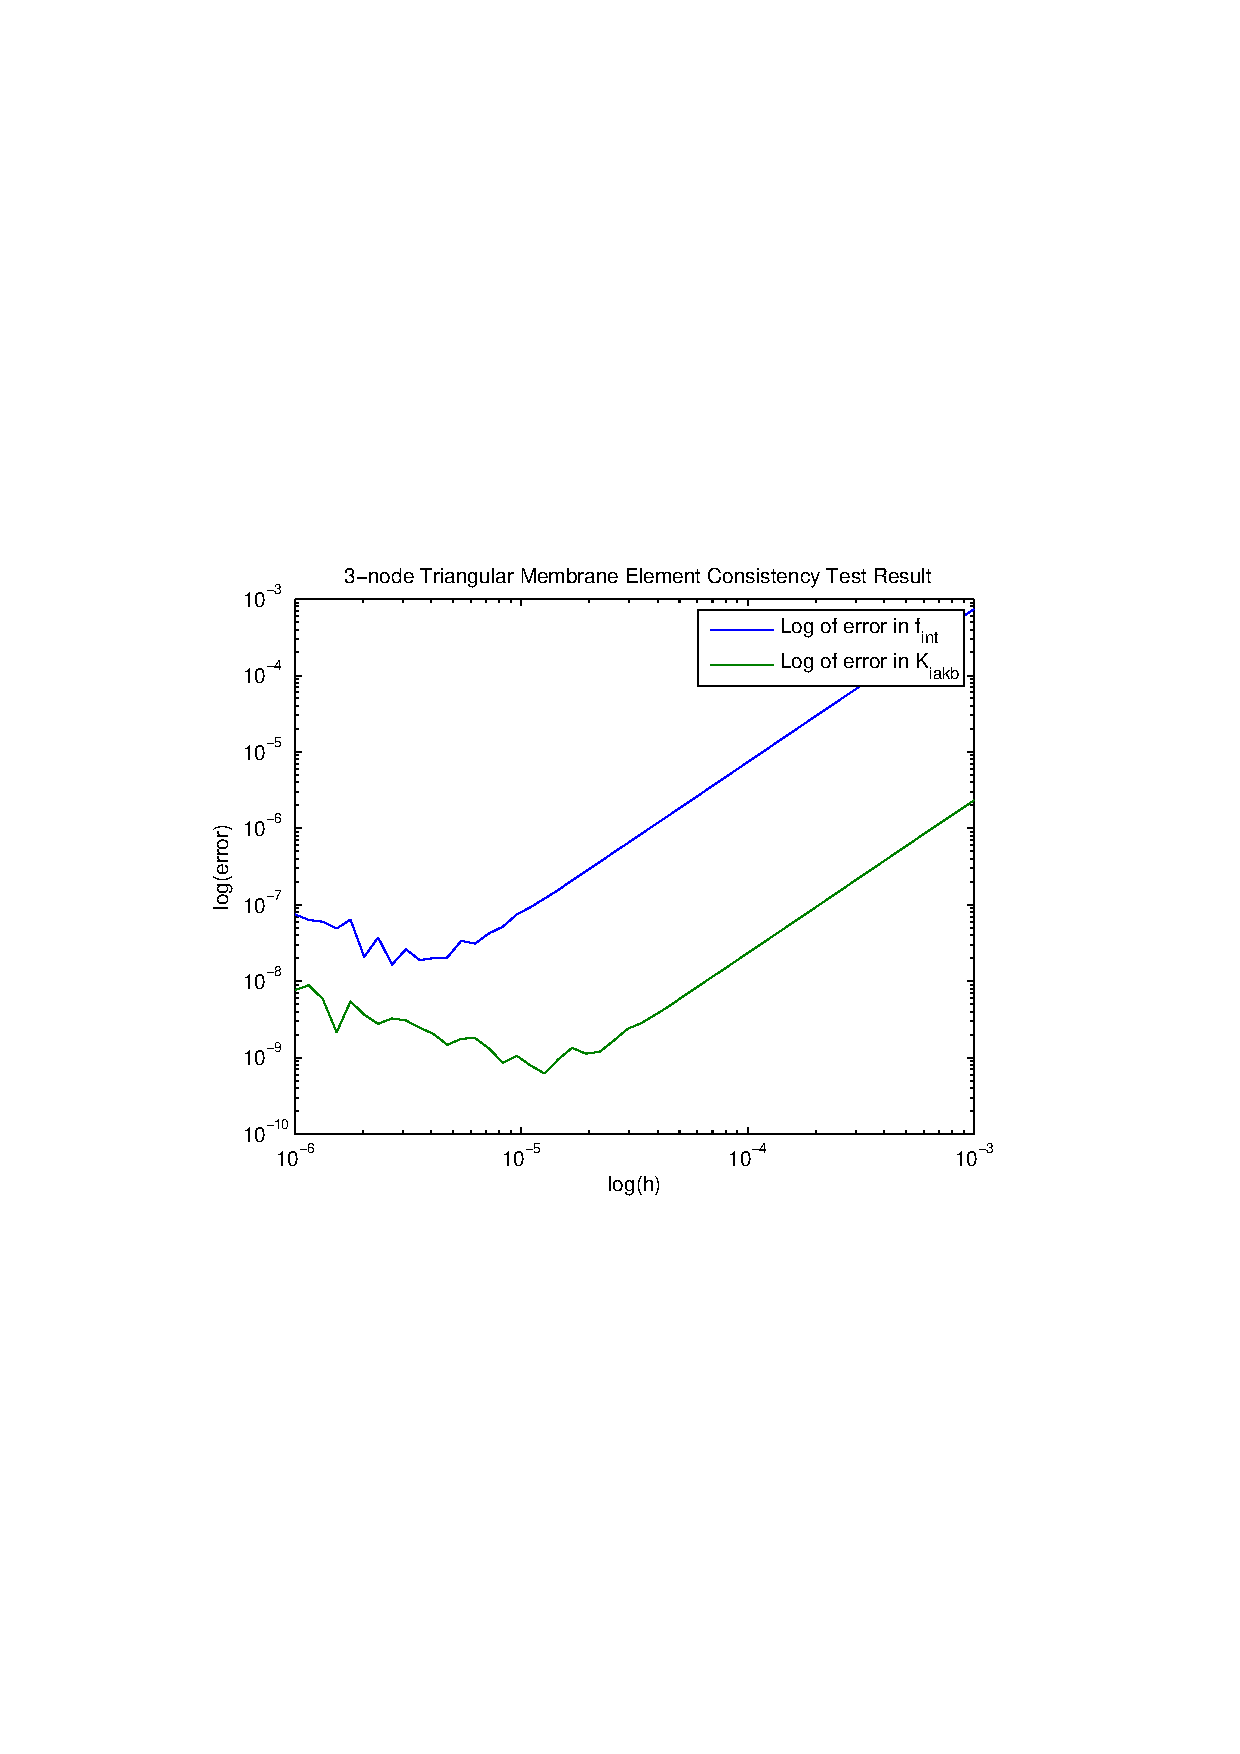
\includegraphics[scale=0.5]{./img/T3MemEle_Consistency.pdf}
    \caption{3-node triangular membrane element}
    \label{fig:linEleCon}
  \end{subfigure}%
  \begin{subfigure}[b]{0.5\textwidth}
    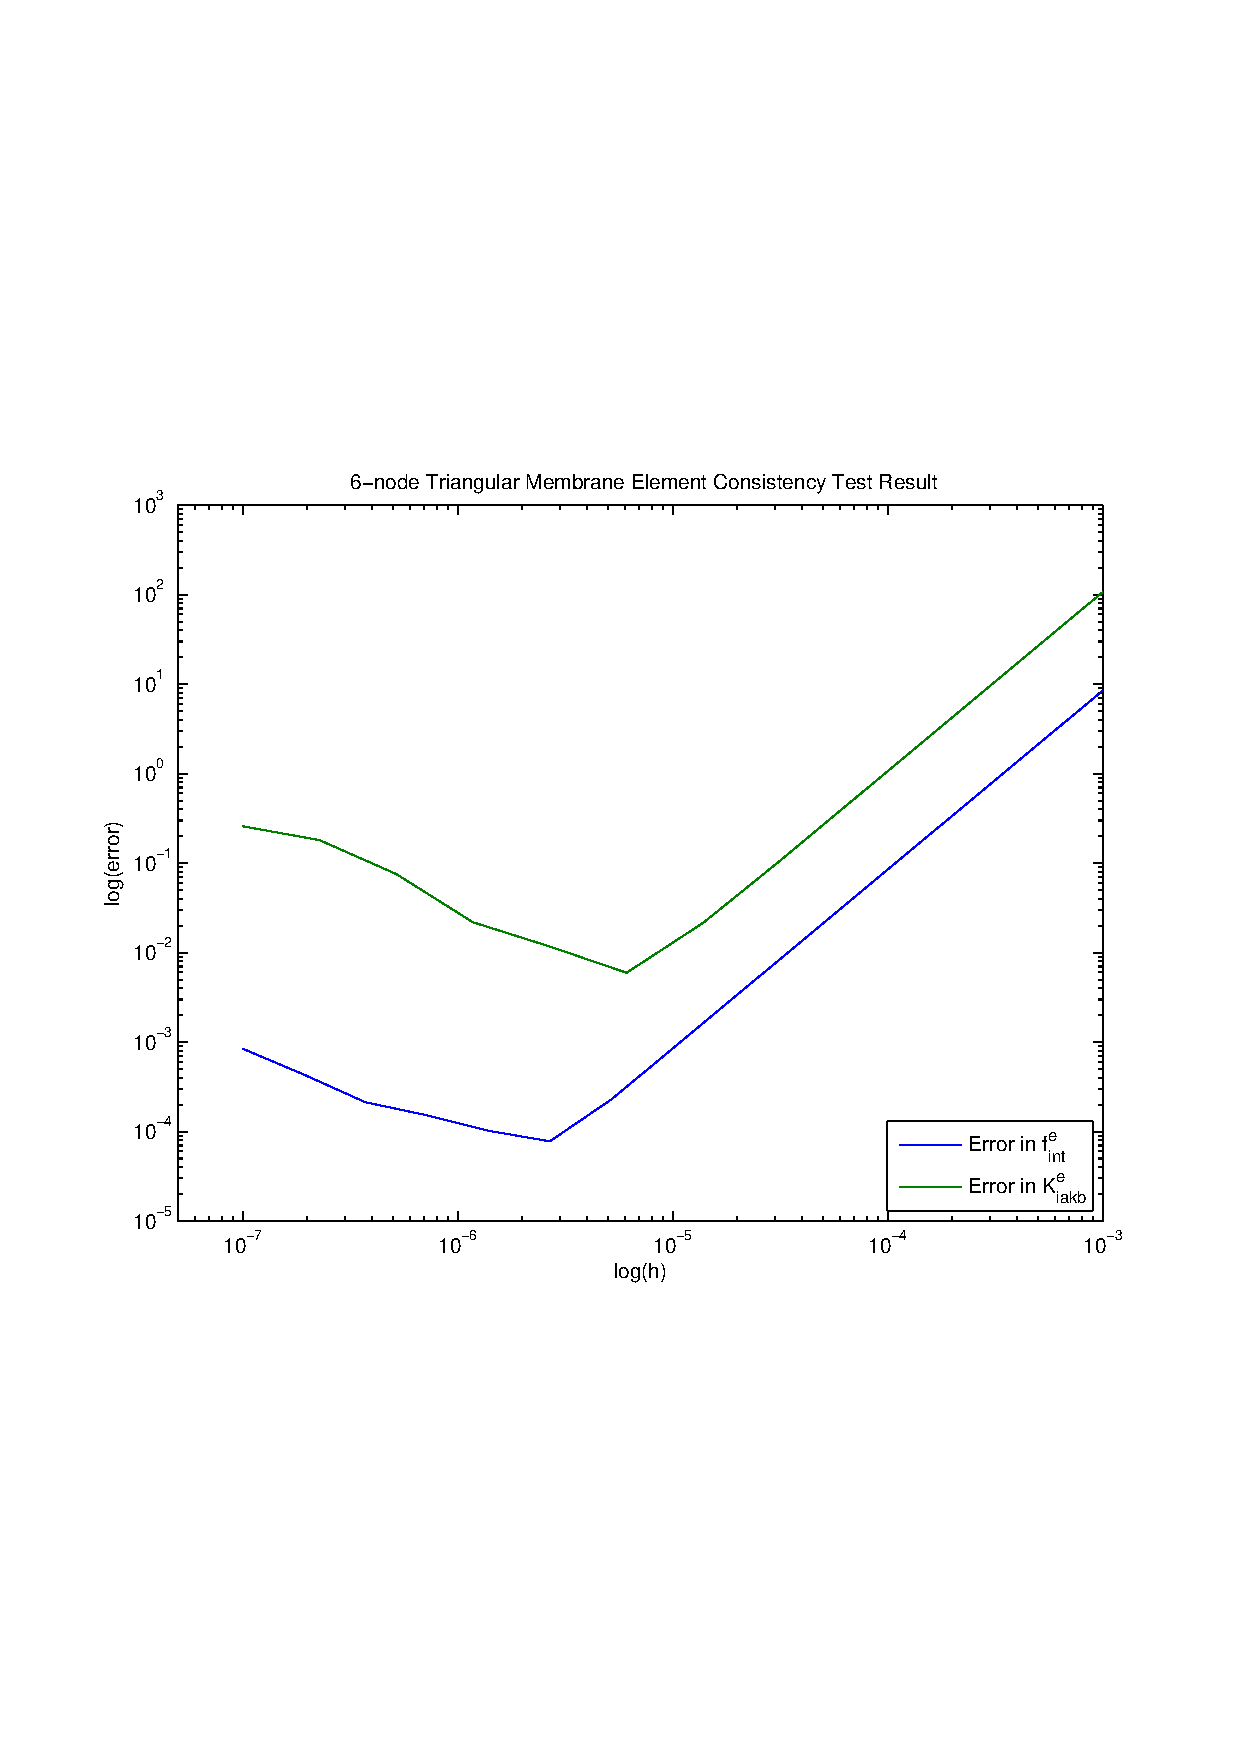
\includegraphics[scale=0.39]{./img/T6MemEle_Consistency.pdf}
    \caption{6-node triangular membrane element}
    \label{fig:quadEleCon}
  \end{subfigure}
  \caption{Log-log plot of error versus $h$ shows straight lines with
    slope 2 indicating error of $\mathcal{O}(h^2)$ as expected for a
    central finite difference numerical differentiation. Smaller vlues
    of $h$ introduce large rounding errors as seen in
    Figure~\ref{fig:linEleCon}}
  \label{fig:eleConsistency}
\end{figure}
\subsubsection{Stiffness Matrix Rank}
The fourth order stiffness modulus $K_{iakb}$ can be \textit{unrolled}
into a square 2-D matrix of size $ia\times kb$. For linear 3-node
triangular element this will give a $9\times9$ matrix and for the
quadratic 6-node triangular element we get a $18\times18$ matrix. We
calculated the rank of the stiffness matrix for the case of zero
deformation i.e. $\mathbf{X}=\mathbf{x}$ and for finite deformation
for both linear and quadratic shape functions. The results are
presented in Table ~\ref{tab:rank}.
\begin{table}
  \centering
  \caption{Rank of stiffness matrix for linear and quadratic membrane elements}
  \label{tab:rank}
  \begin{tabular}{|c|c|c|c|}
    \hline
    Deformation & Shape Function & Quadrature & Rank \\
    \hline
    \multirow{2}{*}{Zero} & Linear & 1-point & 3 \\
    \cline{2-4}                
                & Quadratic & 3-point & 9 \\
    \hline
    \multirow{2}{*}{Finite} & Linear & 1-point & 6 \\
    \cline{2-4}                
                & Quadratic & 3-point & 15 \\
    \hline
  \end{tabular}
\end{table}
In case of zero deformation for 3-node element we have only 1
quadrature points. Thus, in 3-D we have 3 rotational and 3
translational degree of freedom for that point. Hence, the stiffness
matrix is rank-deficient by 6 which gives rank as $9 - 6 = 3$. For
zero-deformation case for 6-node element we have 3 quadrature points
which form a triangle. We need to count number of unique rigid body
motions such that this triangle remains undeformed. We can have 3
rigid-body translations, 3 rotations about the 3 sides of this
triangle and 3 rotations about axis passing through each of the
quadrature point and perpendicular to plane of the triangle. Thus, we
have 9 degrees of freedom. This we should have rank as $18-9=9$. In
case of finite deformation case, the rotational degrees of freedom are
no longer zero-energy modes. So, we expect the rank to increase by 3
and 6 for the 3-node and 6-node elements respectively. Thus, the
results presented in Table ~\ref{tab:rank} are consistent with our
expectations.
\section{Assembly}
In finite element analysis, the geometrical domain of the problem is
discretized into a mesh of finite elements. Our mesh will be using the
finite elements we formulated in the previous section. We need to
compute the combined resultant energy, force and stiffness of the
whole mesh based on contribution from each element. This is done in
the process of assembly in finite element method.
\subsection{Meta Arrays}
We make use of two ``meta'' arrays during the assembly process.
\begin{itemize}
\item \textbf{IEN}: This is the \textit{\textbf{E}lement
    \textbf{N}odes} array. It stores the mesh connectivity
  information. Every node in the mesh is assigned a \textit{global
    node number}. Each row of \textbf{IEN} represents a single
  triangular element in the mesh. The columns of \textbf{IEN} store
  the global node numbers for the vertices of the triangle represented
  by that row. In case of 3-node triangular elements \textbf{IEN} is
  of size $n_{el}\times3$ where $n_{el}$ is the total number of
  elements in the mesh. For the 6-node triangular membrane element the
  size of \textbf{IEN} is $n_{el}\times6$.
\item \textbf{ID}: This is the \textit{\textbf{D}estination} array. It
  stores the \textit{global equation number} corresponding to each
  \textit{global degree of freedom}. For our elements, each node in
  the mesh has 3 degrees of freedom associated with it. We call these
  as the 3 \textit{local degrees of freedom} of each node. Each
  element has $3\times n_{nodes\ per\ element}$ local degrees of
  freedom. So the total number of degrees of freedom in a mesh is
  given by
  \begin{align*}
    \text{Total degrees of freedom} = 3\times \text{total number of nodes}
  \end{align*}
  The degree of freedom numbers associated with a global node numbered
  $a$ can be obtained as
  \begin{align*}
    GDOF(a) = 3(a-1) + i \qquad \text{where}\quad i = 1,2,3
  \end{align*}
  In, each row of \textbf{ID} array the first column is the global
  degree of freedom number and the second column is the \textit{global
    equation number}. If a particular degree of freedom in the mesh is
  constrained due to a prescribed boundary condition then the second
  column in \textbf{ID} array for that global degree of freedom is set
  to 0. \textit{Thus, we assemble the force and stiffness matrices
    only for the unknown degrees of freedom}.
\end{itemize}
\subsection{Potential Energy Assembly}
Total \textit{strain energy} of the mesh is the algebraic sum of
strain energy of each element. The total \textit{potential energy} of
the mesh is the the difference between the total strain energy and the
work done by external forces. Since, we know the external force acting
on each node of each element and we can calculate the nodal
displacements, we can calculate the external work done on the element
as
\begin{align*}
  W^{ext}_e = \mathbf{f}^{ext}_e\cdot\mathbf{u}_e
\end{align*}
Therefore, we can write
\begin{align*}
  \Pi = \sum^{n_{el}}_{e=1}(W^{\text{int}}_e - W^{\text{ext}}_e)
\end{align*}
\subsection{Force Assembly}
Using the \textbf{IEN} and \textbf{ID} arrays, we can get the global
equation number for each local degree of freedom for each
element. Consider the case of 3-node triangular element. It has 9
local degrees of freedom. The element force vectors will be column
vectors with 9 elements, $\mathbf{f}^e$. Suppose the $4^{th}$ local
degree of freedom corresponds to $115^{th}$ global equation
number. Certainly, as the global equation number is non-zero, this is
an unknown degree of freedom and thus we have to assemble its
contribution to the global force matrix, $\mathbf{f}$. The force
(either internal or external) assembly entails that
\begin{align*}
  f_{115} \leftarrow f_{115} + f^{e}_4
\end{align*}
where $\leftarrow$ indicates assignment operation in a computer
program. After assembling both the internal and external forces we can
calculate the global residual force vector as
\begin{align*}
  \mathbf{r} = \mathbf{f}^{\text{int}} - \mathbf{f}^{\text{ext}}
\end{align*}
\subsection{Stiffness Assembly}
Consider the case of 3-node triangular element. It has 9 local degrees
of freedom. The stiffness matrix, $\mathbf{K}^e$ will, therefore, be
of size $9\times9$. Suppose the $4^{th}$ and $6^{th}$ local degrees of
freedom correspond to $115^{th}$ and $227^{th}$ global equation
numbers respectively. Certainly, as the global equation numbers are
non-zero, these are unknown degrees of freedom and thus we have to
assemble their contribution to the global stiffness matrix,
$\mathbf{K}$. The assembly entails that
\begin{align*}
  K_{115,115} &\leftarrow K_{115,115} + K^{e}_{4,4} \\
  K_{115,227} &\leftarrow K_{115,227} + K^{e}_{4,6} \\
  K_{227,115} &\leftarrow K_{227,115} + K^{e}_{6,4} \\
  K_{227,227} &\leftarrow K_{227,227} + K^{e}_{6,6} 
\end{align*}
where $\leftarrow$ indicates assignment operation in a computer
program. Since both $K^e$ and $K$ are symmetric, we could have used
only three assignments instead of four.
\subsection{Verification Tests}
We will test our implementation for bugs using consistency test and by
checking the rank of stiffness matrix for zero and finite
deformations.
\subsubsection{Consistency Test}
The global potential energy $\Pi$, residual force $\mathbf{r}$ and the
global stiffness modulus $\mathbf{K}$ are inter-related as
\begin{align*}
  r_{ia} &=\frac{\partial\Pi}{\partial x_{ia}} \\
  K_{iakb} &= \frac{\partial r_{ia}}{\partial x_{kb}}
\end{align*}
We can use these to test our implementation by comparing the results
obtained from our assembly sub-routine with the numerical derivatives
calculated using 3-point finite difference scheme. The equations for
numerical derivatives are
\begin{align*}
  r_{ia} &\approx \frac{W(x_{ia}+h) - W(x_{ia}-h)}{2h}\\
  K_{iakb} &\approx \frac{r_{ia}(x_{kb}+h)-r_{ia}(x_{kb}-h)}{2h}
\end{align*}
We chose several values for perturbation $h \in (10^{-7},10^{-3})$.
The error in the numerical derivatives scaled quadratically with $h$
as can be seen from Figure~\ref{fig:assyConsistency}.
\begin{figure}[ht]
  \centering
  \begin{subfigure}[b]{0.5\textwidth}
    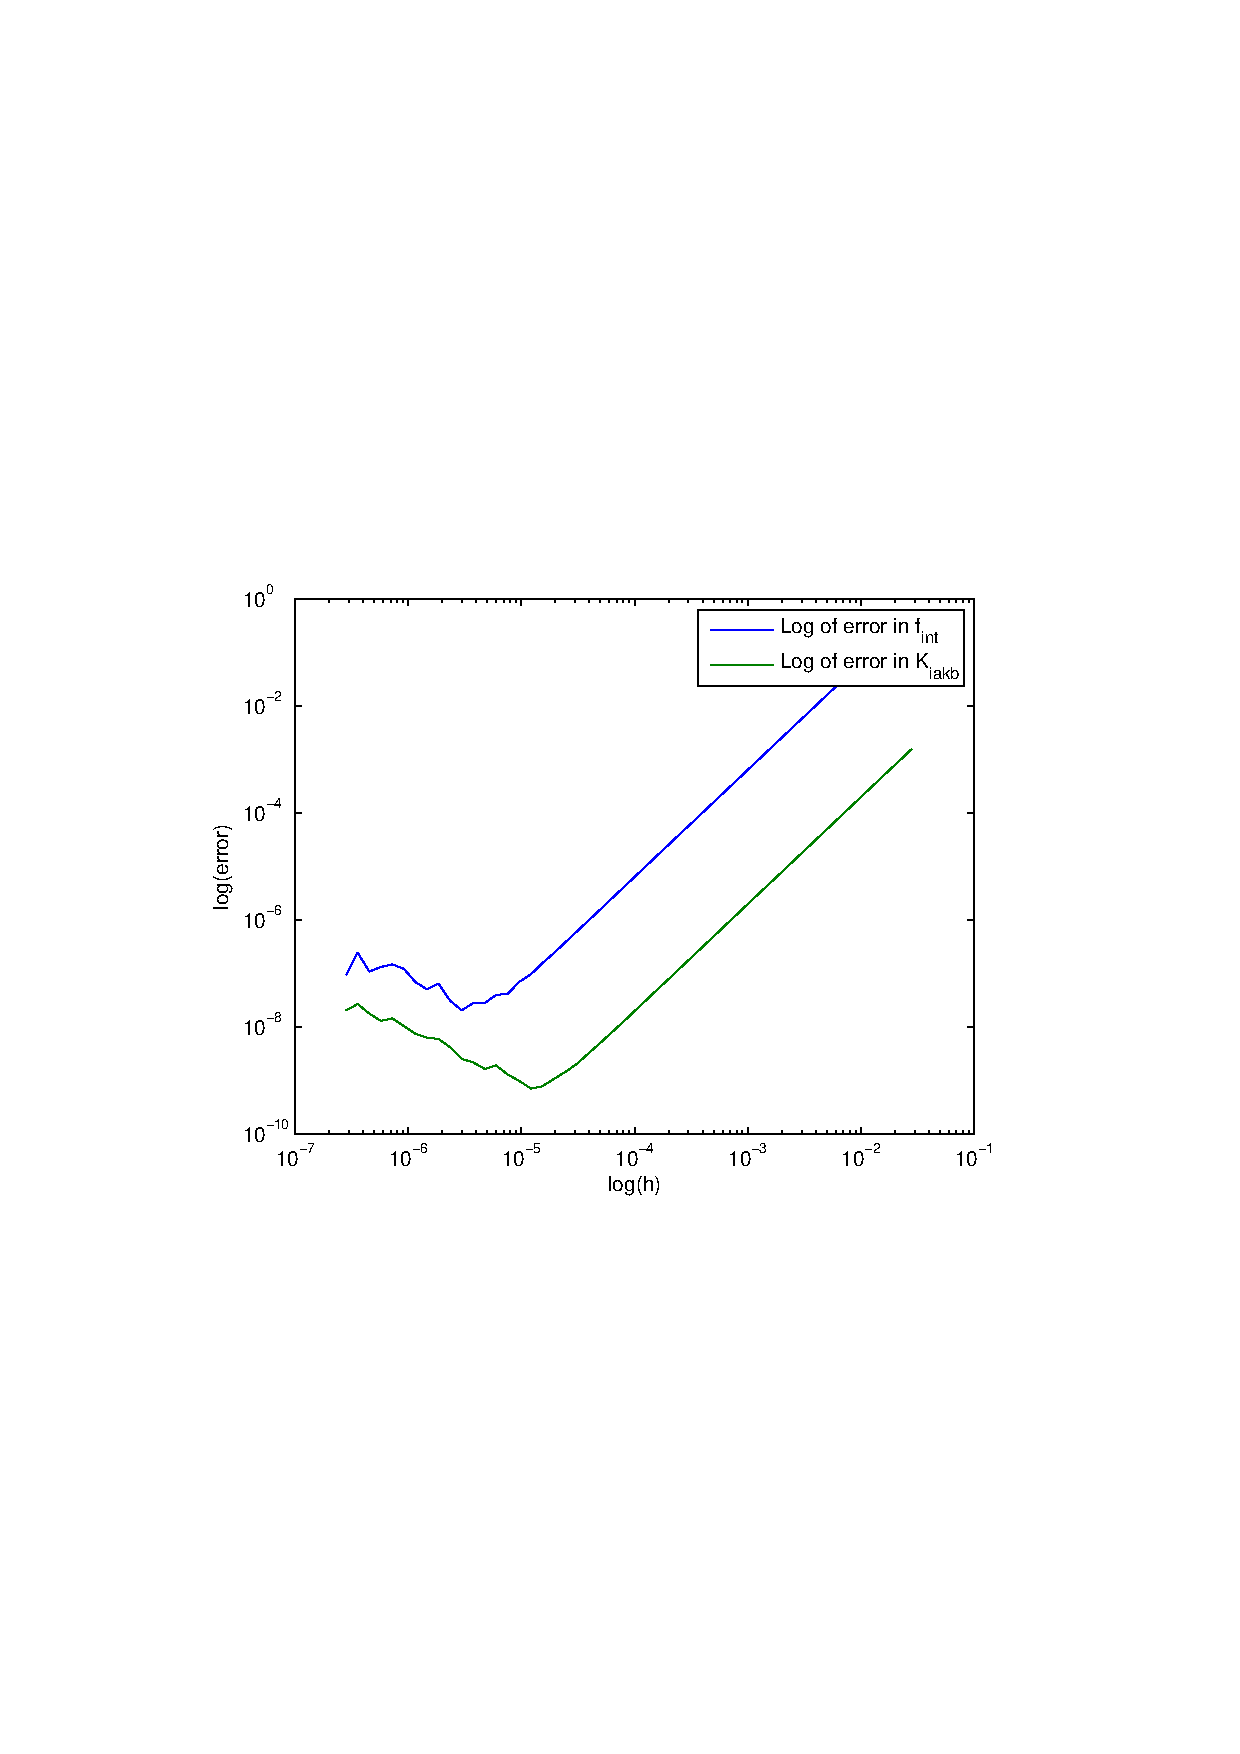
\includegraphics[scale=0.5]{./img/T3AssyConsistency.pdf}
    \caption{Assembly of 3-node triangular elements}
    \label{fig:linAssyCon}
  \end{subfigure}%
  \begin{subfigure}[b]{0.5\textwidth}
    \includegraphics[scale=0.5]{./img/T6AssyConsistency.pdf}
    \caption{Assembly of 6-node triangular elements}
    \label{fig:quadAssyCon}
  \end{subfigure}
  \caption{Log-log plot of error versus $h$ shows straight lines with
    slope 2 indicating error of $\mathcal{O}(h^2)$ as expected for a
    central finite difference numerical differentiation. Smaller vlues
    of $h$ introduce large rounding errors.}
  \label{fig:assyConsistency}
\end{figure}
\subsubsection{Rank of Stiffness Matrix}
The global stiffness matrix is a square matrix with number of rows and
columns equal to the number of unknown global degrees of freedom. We
chose a square mesh of two triangular elements, as shown in
Figure~\ref{fig:assyStiffRankMesh} and constrained one of the corner
nodes to have zero displacement in all three directions. Then we
prescribed zero and finite displacements for other nodes of the
element and calculated the rank of stiffness matrix in both cases. We
did this for both the 3-node and the 6-node element. The results are
summarized in the table ~\ref{tab:assyStiffness}
\begin{table}
  \centering
  \caption{Rank of Global Stiffness matrix after assembly for Linear and Quadratic membrane elements}
  \label{tab:assyStiffness}
  \begin{tabular}{|c|c|c|}
    \hline
    Shape Function & Deformation &  Rank \\
    \hline
    \multirow{2}{*}{Linear} & Zero & 9 \\
    \cline{2-3}                
                   & Finite & 9 \\
    \hline
    \multirow{2}{*}{Quadratic} & Zero & 24 \\
    \cline{2-3}                
                   & Finite & 24 \\
    \hline
  \end{tabular}
\end{table}
\begin{figure}[ht]
  \centering
  \begin{subfigure}[b]{0.5\textwidth}
    \includegraphics[scale=0.52]{./img/assyStiffRankMesh3.pdf}
    \caption{Mesh of 3-node elements}
    \label{fig:linAssyStiffRank}
  \end{subfigure}%
  \begin{subfigure}[b]{0.5\textwidth}
    \includegraphics[scale=0.39]{./img/assyStiffRankMesh6.pdf}
    \caption{Mesh of 6-node elements}
    \label{fig:quadAssyStiffRank}
  \end{subfigure}
  \caption{Meshes used to verify the rank of stiffness matrix obtained
    after assembly. The nodes in the mesh have been circled.}
  \label{fig:assyStiffRankMesh}
\end{figure}
For the 3-node element mesh, there are 4 global nodes and 12 global
degrees of freedom. We have constrained 3 of these degrees of
freedom. So we are left with 9 unknown degrees of freedom. Each row
and column of the $9\times9$ assembled stiffness matrix corresponds to
one of the unknown degree of freedom. Since, we want our system of
equations to give us a unique answer for each unknown degree of
freedom we expect that the assembled stiffness matrix has full
rank. In our example, it should have rank 9. Similar, analysis for the
mesh of 6-node elements shows that we should expect the assembled
stiffness matrix to have rank 24. The results shown in Table
~\ref{tab:assyStiffness} are thus consistent with our expectations. It
is very important to highlight at this point that in the zero
deformation case, it was necessary to perturb the unconstrained
degrees of freedom in the transverse direction by a small
amount. Otherwise, the membrane mesh would be perfectly flat and offer
no resistance in the transverse direction giving rise to unwanted rank
deficiency in the stiffness matrix.
\section{Solving the Equilibrium Problem}
The object of our finite element analysis is to calculate nodal
displacements that lead to the system being in equilibrium
characterized by zero residual force vector. The residual force vector
is a non-linear function of the current configuration and we can use
Newton-Raphson method to solve for equilibrium displacement as follows
\subsection{Newton-Raphson Method for Equilibrium}
\begin{align*}
  \mathbf{r}(\mathbf{x+\mathbf{u}}) &\approx \mathbf{r}(\mathbf{x}) + \frac{\partial\mathbf{r}}{\partial\mathbf{x}}\mathbf{u} \\
                                    &= \mathbf{r}(\mathbf{x}) + \mathbf{K}\mathbf{u}
\end{align*}
We want $ \mathbf{r}(\mathbf{x+\mathbf{u}}) = 0$, therefore,
\begin{align*}
  \mathbf{u} = \mathbf{K}^{-1}\mathbf{r}
\end{align*}
The $\mathbf{u}$ represents the update required to our current guess
for $\mathbf{x}$. We repeat this till the residual is driven to zero
to acceptable numerical tolerance.
\subsection{Incremental Solution Strategy}
When the mesh is subjected to relatively large forces or
displacements, the Newton iterations will not converge unless we have
a very good initial guess. To resolve this problem we can adopt an
incremental solution strategy. We can divide the total prescribed
force or displacement in small increments such that for the first
increment from zero our Newton iterations for equilibrium converge
with the reference configuration itself as our initial guess for the
solution. For subsequent increments in load (force or displacement) we
can use the solution obtained for the previous increment as the
initial guess.

\section{Applications}
\subsection{Planar Isotropic Stretch}
We have to solve the problem of a square sheet stretched by a planar
isotropic deformation($F_{11}=F_{22}=\lambda,F_{12}=F_{21}=0$) imposed
by prescribing displacements of nodes on the
boundaries. Figure~\ref{fig:equiBiaxialMesh} shows the reference and
deformed configuration mesh, obtained by our finite element analysis,
superimposed.
\begin{figure}[h]
  \centering
  \includegraphics[scale=0.5]{./img/equiBiaxialMesh.pdf}
  \caption{The reference configuration mesh has been superimposed on
    the deformed mesh. Brown mesh represents the reference
    configuration and blue mesh represents the deformed configuration
    obtained by our finite element analysis. The square sheet has
    stretched isotropically as expected. }
  \label{fig:equiBiaxialMesh}
\end{figure}
Using the incremental solution strategy discussed in previous section,
we solved for the deformed configuration for various planar isotropic
stretches and compressions of the initial mesh. As a post-processing
step for every isotropic stretch, we calculated the mean deformation
gradient for all elements and checked if the deformation gradient for
any element deviated significantly from the mean. In all cases, the
deviation was within numerical tolerance and thus we found that the
deformation gradient was uniform across the mesh.
\begin{figure}[h]
  \centering
  \includegraphics[scale=0.75]{./img/EquiBiaxial.pdf}
  \caption{$P_{11}$ and $P_{22}$ components of first Piola-Kirchhoff
    stress tensor plotted against a component of deformation gradient
    $F_{11}$. This result is same as obtained in HW 1 for compressible
    neo Hookean material.}
  \label{fig:equiBiaxialStressStrain}
\end{figure}
It should be noted that we had to prescribe the transverse
displacement of all nodes to be zero. Otherwise, as the reference
configuration is a perfectly flat mesh, the stiffness matrix has zero
stiffness components in the transverse direction which leads to a
singular matrix that cannot be inverted as required for our
equilibrium Newton iterations. By prescribing the transverse
displacement we ensure that those degrees of freedom are not assembled
into our global stiffness matrix.
\subsection{Simply Supported Membrane under Transverse Load}
We have to solve the problem of a simply supported square membrane
under a uniform transverse load. Side length of the square mesh was
chosen to be $L = 10\ cm$. Reference thickness $H = 0.1\ cm$, shear
modulus, $\mu_0 = 4\times10^5\ N/m^2$ and $\lambda_0 = 10\mu_0$. We
will use incremental solution strategy for applied transverse load. We
will increase it in increments of $10\ N/m^2$ from $0$ to
$1000\ N/m^2$.
\begin{figure}[ht]
  \centering
  \begin{subfigure}[b]{0.3\textwidth}
    \includegraphics[scale=0.3]{./img/initialMesh.pdf}
    \caption{Undeformed mesh, 200 elements}
    \label{fig:prob3initialMesh}
  \end{subfigure}%
  \begin{subfigure}[b]{0.3\textwidth}
    \includegraphics[scale=0.3]{./img/halfDeformedMesh.pdf}
    \caption{Deformed mesh under half of maximum load}
    \label{fig:prob3HalfDeformedMesh}
  \end{subfigure}
  \begin{subfigure}[b]{0.3\textwidth}
    \includegraphics[scale=0.3]{./img/deformedMesh.pdf}
    \caption{Deformed mesh under maximum load}
    \label{fig:prob3FullDeformedMesh}
  \end{subfigure}
  \caption{The reference configuration mesh and the deformed mesh at
    half load and full load using 3-node triangular membrane elements
    are shown. The maximum deflection at half load is only slightly
    less than the deflection at full-load.}
  \label{fig:prob3Mesh}
\end{figure}
Figure~\ref{fig:prob3Mesh} shows the mesh at zero, half the maximum
and the maximum load full load. We can observe that the deformed mesh
at half-load is almost identical to the deformed mesh at full load. It
indicates that the increase in deflection goes on decreasing rapidly
as the transverse load increases. This is expected because as the
membrane deflects under the transverse load its area increases and it
has to stretch. The more it stretches, the stiffer it becomes and thus
it takes larger force to stretch it further. This relationshiip
between maximum deflection andthe transverse load can also be noticed
in Figure~\ref{fig:forceDeflection}.
\begin{figure}[ht]
  \centering
  \begin{subfigure}[b]{0.3\textwidth}
    \includegraphics[scale=0.3]{./img/initialMeshT6.pdf}
    \caption{Top view of undeformed mesh, 50 elements}
    \label{fig:prob3initialMeshT6}
  \end{subfigure}%
  \begin{subfigure}[b]{0.3\textwidth}
    \includegraphics[scale=0.3]{./img/halfDeformedMeshT6.pdf}
    \caption{Deformed mesh under half of maximum load}
    \label{fig:prob3DeformedMeshT6}
  \end{subfigure}
  \begin{subfigure}[b]{0.3\textwidth}
    \includegraphics[scale=0.3]{./img/deformedMeshT6.pdf}
    \caption{Deformed mesh under maximum load}
    \label{fig:prob3DeformedMeshT6}
  \end{subfigure}
  \caption{The reference configuration mesh and the deformed mesh at
    half load and full load using 6-node triangular membrane elements
    are shown. The deformed mesh plots are misleading because the
    triangles in the mesh don't show the mid-side nodes.}
  \label{fig:prob3MeshT6}
\end{figure}
Figure~\ref{fig:prob3MeshT6} shows the mesh of 6-node triangular
membrane elements at zero, half of the maximum and maximum transverse
load. Figure~\ref{fig:prob3initialMeshT6} is the top-view of the
initial mesh. It also shows the mid-side nodes. 6-node triangular
elements have mid-side nodes which make the sides of the triangle
quadratic functions instead of straight lines. But this detail is
missing from Figure~\ref{fig:prob3MeshT6}. A better representation of
the displacement field is shown in
Figure~\ref{fig:deformedMeshRefined}. It is obtained by doing a
Delaunay triangulation of the cloud of points formed by the nodes of
the original mesh and then plotting the displacement field over
it. Like Figure~\ref{fig:prob3Mesh}, this representation also has the
drawback that the triangles in the mesh are not actually the elements
but it gives better visualization of the displacement field. 6-node
quadratic element mesh gives more accurate solution with lesser number
of elements as compared to the mesh of 3-node triangular elements.
\begin{figure}[h]
  \centering
  \includegraphics[scale=0.5]{./img/deformedMeshRefined.pdf}
  \caption{Alternative representation of deformed 6-node triangular
    element mesh. But the triangles in this figure are not the
    elements.}
  \label{fig:deformedMeshRefined}
\end{figure}
\begin{figure}[ht]
  \centering
  \begin{subfigure}[b]{0.5\textwidth}
    \includegraphics[scale=0.5]{./img/forceDeflection.pdf}
    \caption{For 3-node element mesh}
    \label{fig:fDT3}
  \end{subfigure}%
  \begin{subfigure}[b]{0.5\textwidth}
    \includegraphics[scale=0.5]{./img/forceDeflectionT6.pdf}
    \caption{For 6-node elements mesh}
    \label{fig:fDT6}
  \end{subfigure}
  \caption{Force-deflection curve for the 3-node and 6-node element
    meshes. The slope decreases as the maximum deflection
    increases. This shows that it requires more force to bring about
    equal increase in maximum deflection as the membrane deforms.}
  \label{fig:forceDeflection}
\end{figure}
\subsection{Spherical balloon}
We have to sovle the problem of a spherical balloon of initial radius
$R=10\ cm$ and thickness $H = 0.1\ cm$ under a uniform internal
pressure. We used incremental solution strategy as before. The initial
mesh and several deformed mesh are shown in
Figure~\ref{fig:balloonMesh}.
\begin{figure}[ht]
  \centering
  \begin{subfigure}[b]{0.5\textwidth}
    \includegraphics[scale=0.5]{./img/balloon.pdf}
    \caption{Initial Mesh of radius $R=10\ cm$}
    \label{fig:initialBalloon}
  \end{subfigure}%
  \begin{subfigure}[b]{0.5\textwidth}
    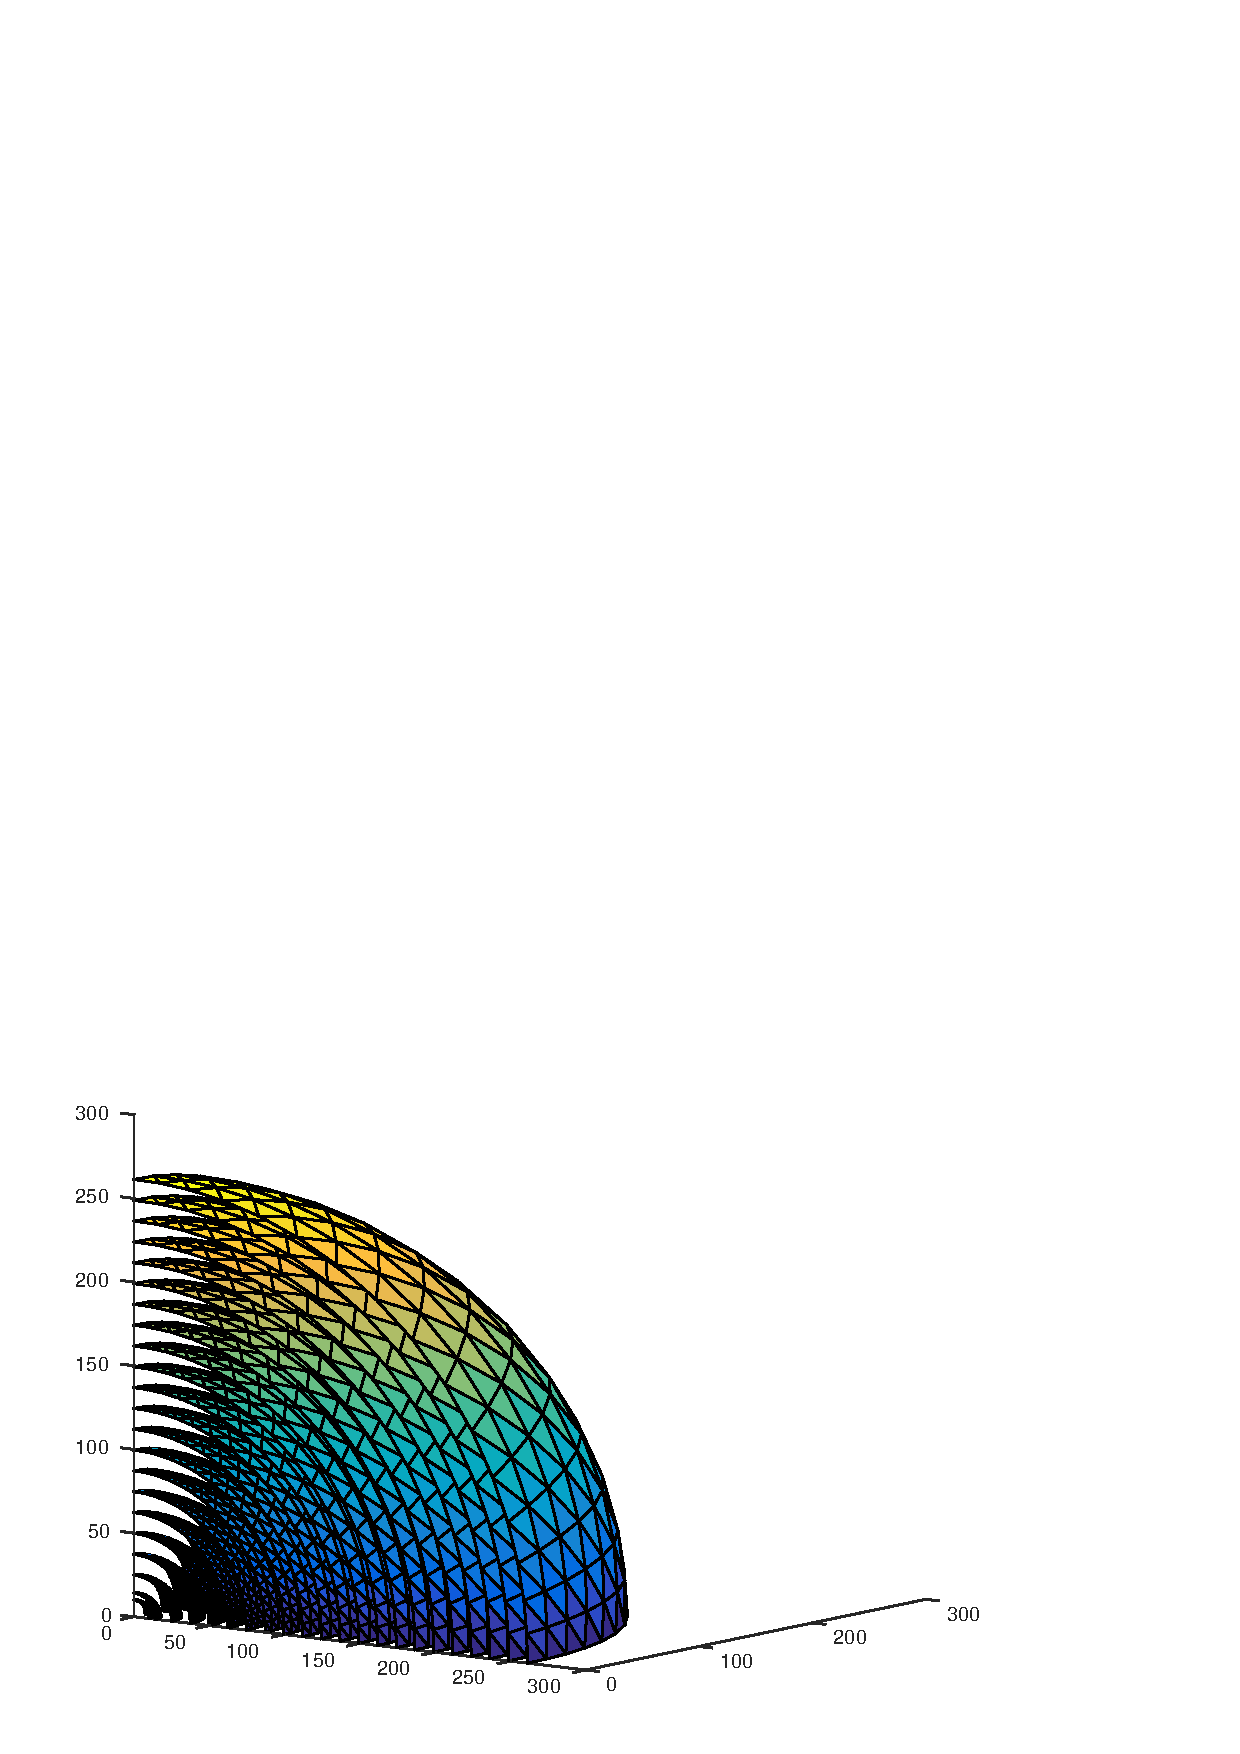
\includegraphics[scale=0.5]{./img/balloonBlowingUp2.pdf}
    \caption{Several deformed mesh of increasing radii}
    \label{fig:deformedBalloons}
  \end{subfigure}
  \caption{The initial mesh and many deformed meshes of an octant of a
    spherical membrane subjected to uniform internal pressure.}
  \label{fig:balloonMesh}
\end{figure}
Figure~\ref{fig:pressStretch} shows the variation in stretch-ratio
defined as $\lambda=r/R$ where $r$ and $R$ are the current and
reference configuration radii. The plot is similar to
Figure~\ref{fig:equiBiaxialStressStrain}. The Newton-Raphson
iterations for enforcing plane-stress at element level could not drive
the normal component of traction vector below $1\times10^{-6}$ after a
pressure of $60\ N/m^2$ because the Newton updates became of the order
of machine precision. But as the component is still much smaller than
the traction vector in the plane of membrane, we continued to solve
for equilibrium for larger pressures till $220\ N/m^2$ when the Newton
iterations for the equilibrium stopped converging.
\begin{figure}[h!]
  \centering
  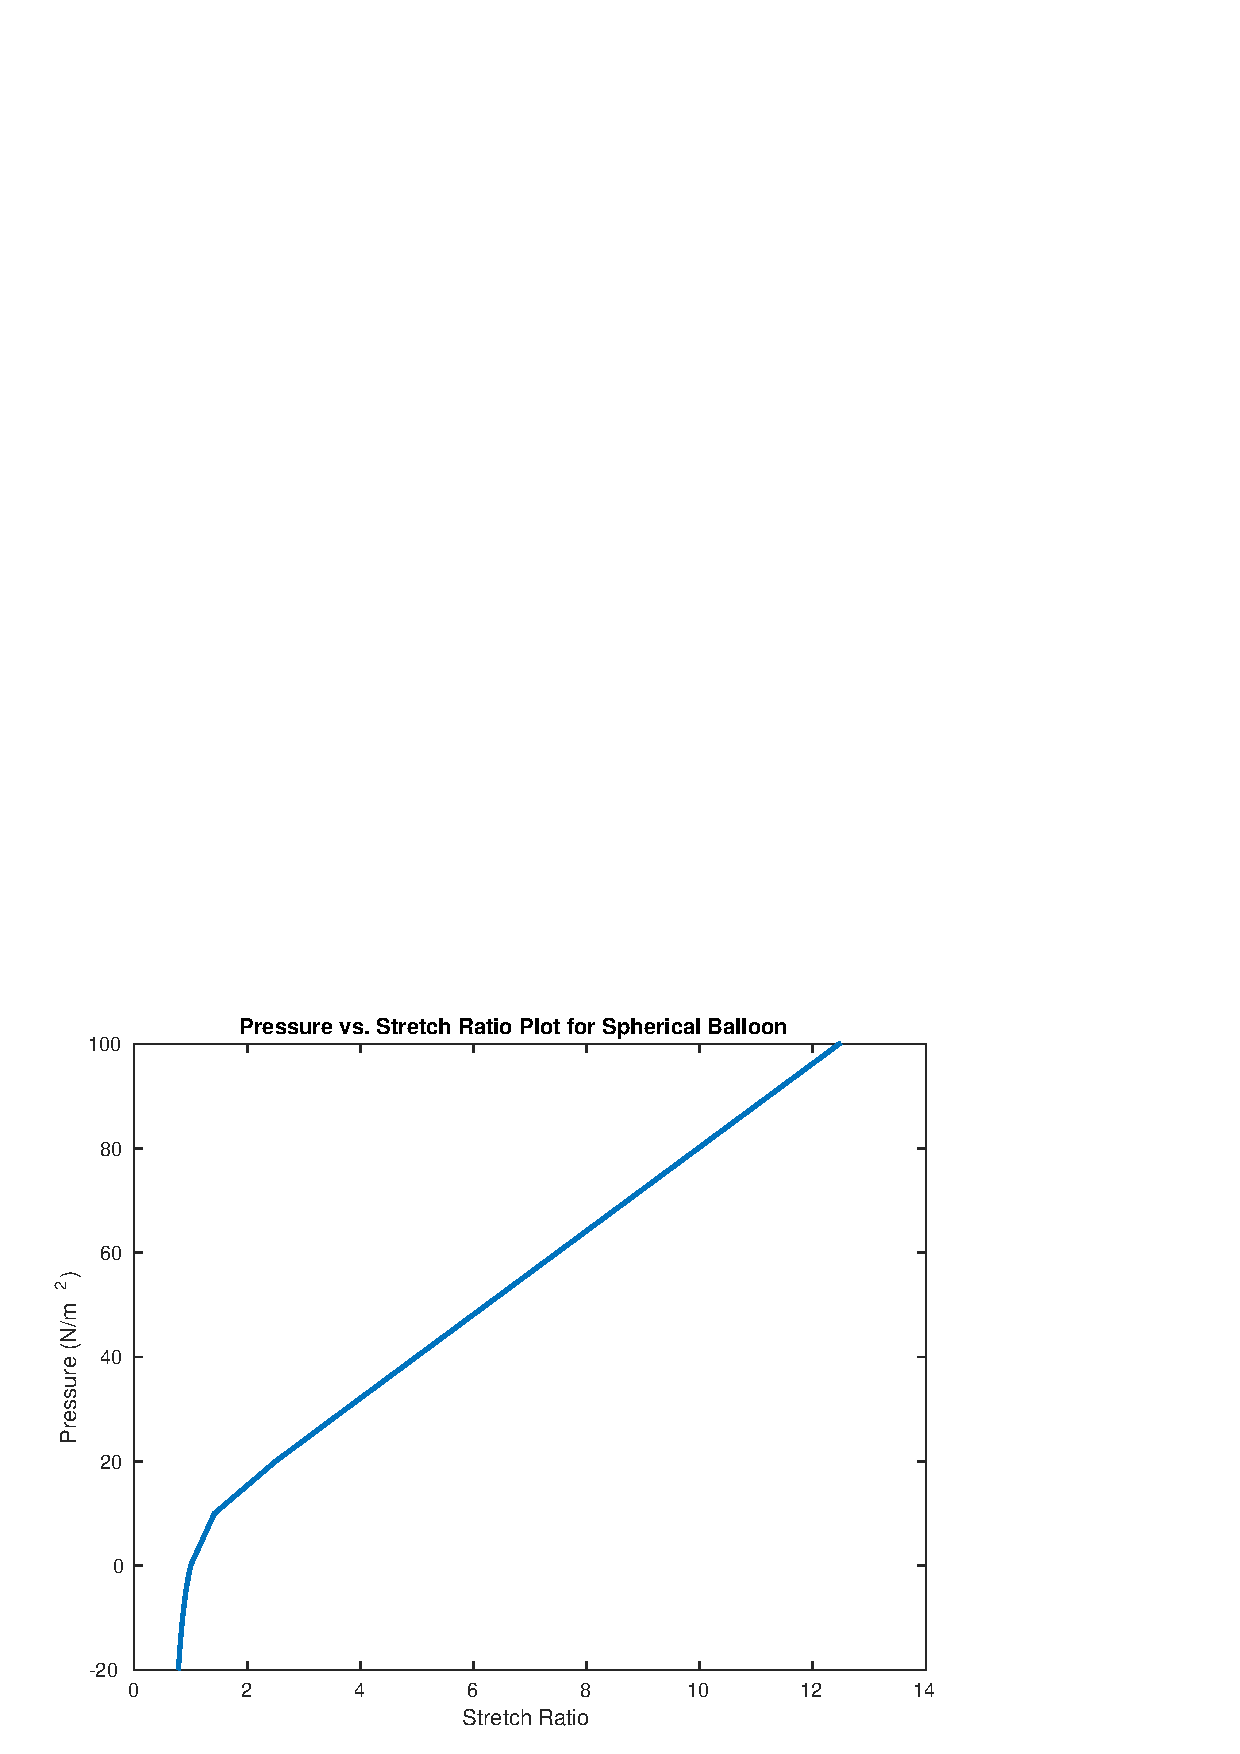
\includegraphics[scale=0.75]{./img/pressureStretch.pdf}
  \caption{Pressure versus stretch-ratio plot for the balloon
    problem. It shows similar behavior as the equibiaxial strain
    problem in Figure~\ref{fig:equiBiaxialStressStrain}}
  \label{fig:pressStretch}
\end{figure}

\section{Source Code Listing}
\begin{itemize}
\item \texttt{assemblyT3Lin.m}: This function performs assembly for a
  mesh of 3-node triangular membrane elements.
\item \texttt{assemblyT6Quad.m}: This function performs assembly for a
  mesh of 6-node triangular membrane elements.
\item \texttt{BalloonProblem.m} This is the driver script from the
  balloon problem.
\item \texttt{calcAllCs.m}: This function performs the plane-stress
  enforcement at element level and calculates various stiffness moduli
  required to calculate the membrane element stiffness modulus.
\item \texttt{calcFandP.m}: This function is a post-processing
  function used to calculate deformation gradient and first
  Piola-Kirchoff stress tensor. It is used to check for uniform
  deformation gradient.
\item \texttt{convertToT6Mesh.m}: This function is used to add
  mid-side nodes to a 3-node triangular element mesh and regenerate a
  connectivity matrix to get a 6-node triangular element mesh.
\item \texttt{EquibiaxialStrain.m}: This is the driver script for the
  isotropic stretch problem.
\item \texttt{equiTriMesh.m}: This fucntion creates a mesh of
  triangles in a large equilateral triangles. It is used to generate
  the spherical balloon octant mesh.
\item \texttt{findStiffnessRank.m}: This function calculates rank of a
  matrix.
\item \texttt{getBCmatrix.m}: This function accepts a cell-array
  containing infformation about boundary condition in terms of nodal
  co-ordinates and local degree of freedom for a mesh and generates a
  matrix containing the boundary condition specified with respect to
  global degree of freedom number.
\item \texttt{neoHookean.m}: This function calculates the strain
  energy density, first Piola-Kirchhoff stress tensor and the
  corresponding tangent modulus.
\item \texttt{plotMesh.m}: This function generates a 3-D plot of a
  mesh and saves it to file.
\item \texttt{plotQuiver.m}: This function plots force vector field on
  a mesh for visualization.
\item \texttt{Element\_Stiffness\_rank.m}: This script calculates the
  rank of stiffness matrix for 3-node and 6-node membrane elements
  under zero or finite deformations.
\item \texttt{T3\_assy\_consistency\_check.m}: This script performs
  consistency check for \texttt{assemblyT3Lin.m}
\item \texttt{T3\_assy\_Stiffness\_Rank.m}: This script calculates the
  stiffness rank for 3-node triangular element mesh under zero and
  finite deformation.
\item \texttt{T3Lin.m}: This function calcuates the 3-node linear
  triangular shape functions and its derivatives.
\item \texttt{T3MembraneEle.m}: This function calculates strain
  energy, nodal force vectors and stiffness modulus for a 3-node
  triangular membrane element.
\item \texttt{T3MembraneEle\_Verification.m}: This script checks
  \texttt{T3MembraneEle.m} for consistency.
\item \texttt{T6\_assy\_consistency\_check.m}: This script performs
  consistency check for \texttt{assemblyT6Quad.m}
\item \texttt{T6\_assy\_Stiffness\_Rank.m}: This script calculates the
  stiffness rank for 6-node triangular element mesh under zero and
  finite deformation.
\item \texttt{T6Quad.m}: This function calcuates the 6-node linear
  triangular shape functions and its derivatives.
\item \texttt{T6MembraneEle.m}: This function calculates strain
  energy, nodal force vectors and stiffness modulus for a 6-node
  triangular membrane element.
\item \texttt{T6MembraneEle\_Verification.m}: This script checks
  \texttt{T6MembraneEle.m} for consistency.
\item \texttt{TransverseLoadExample.m}: This is the driver script for
  transverse load problem.
\item \texttt{TriGaussQuad.m}: Returns the Gauss-quadrature points and
  weights for 1-point and 3-point schemes.
\end{itemize}
\end{document}
